\documentclass[tikz,border=6pt]{standalone}
\usepackage[T1]{fontenc}
\usepackage{lmodern}
\usepackage{amsmath}
\usetikzlibrary{positioning,arrows.meta,fit,backgrounds,calc}
\definecolor{c1}{HTML}{30638E}
\definecolor{c3}{HTML}{D1495B}
\definecolor{c5}{HTML}{66A182}
\definecolor{g}{HTML}{BBBBBB}
\begin{document}
\sffamily\small
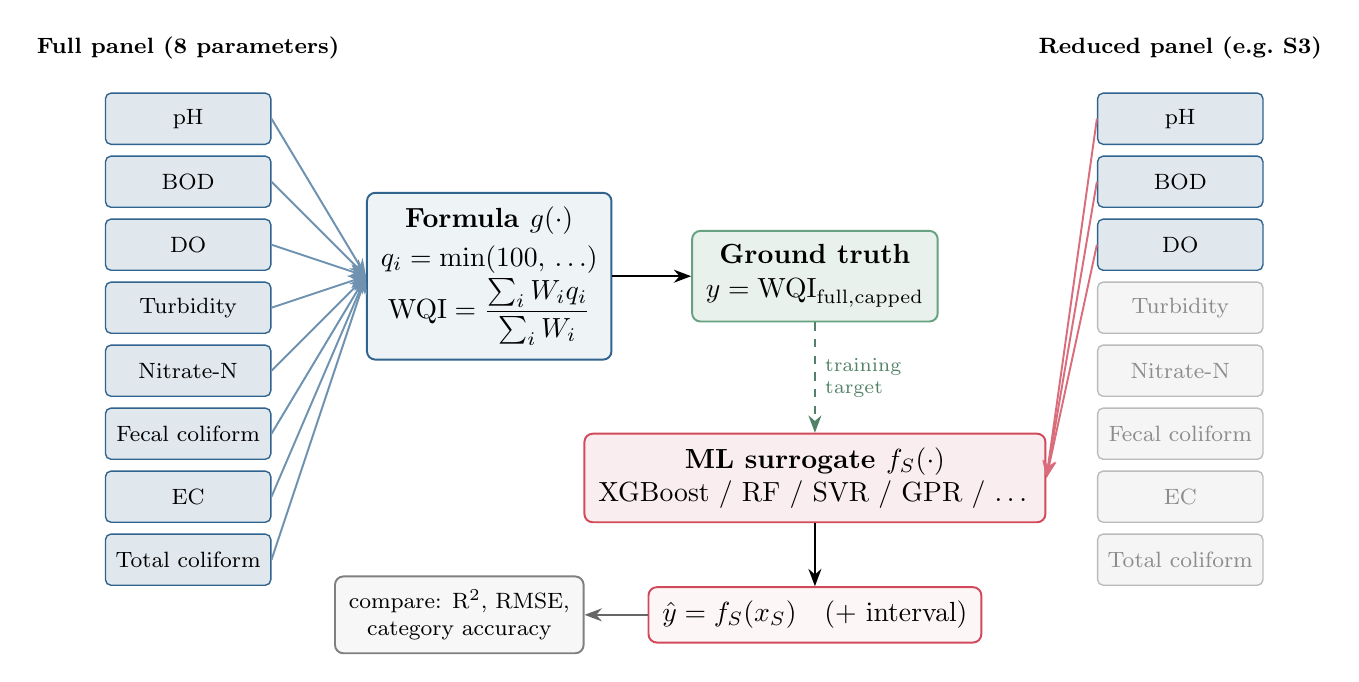
\begin{tikzpicture}[
  p/.style={draw, rounded corners=2pt, minimum width=21mm, minimum height=6.5mm, font=\footnotesize, line width=0.5pt},
  on/.style={p, fill=c1!15, draw=c1},
  off/.style={p, fill=black!4, draw=g, text=black!45},
  box/.style={draw, rounded corners=3pt, align=center, line width=0.7pt, inner sep=5pt},
  arr/.style={-{Stealth[length=2.2mm]}, line width=0.7pt}
]
% left: full panel
\foreach \n/\lbl [count=\i] in {pH/pH, BOD/BOD, DO/DO, Tu/Turbidity, Ni/Nitrate-N, FC/Fecal coliform, EC/EC, TC/Total coliform}{
  \node[on] (L\n) at (0,-\i*0.8) {\lbl};
}
\node[box, fill=c1!8, draw=c1, right=12mm of LTu, yshift=4mm] (g) {\textbf{Formula $g(\cdot)$}\\[2pt] $q_i=\min(100,\,\ldots)$\\[1pt] $\mathrm{WQI}=\dfrac{\sum_i W_i q_i}{\sum_i W_i}$};
\foreach \n in {pH,BOD,DO,Tu,Ni,FC,EC,TC}{ \draw[arr, c1!70] (L\n.east) -- (g.west); }
\node[box, fill=c5!15, draw=c5, right=10mm of g] (y) {\textbf{Ground truth}\\$y=\mathrm{WQI}_{\text{full,capped}}$};
\draw[arr] (g) -- (y);
\node[font=\footnotesize\bfseries, above=3mm of LpH] {Full panel (8 parameters)};

% right: reduced
\foreach \n/\lbl/\st [count=\i] in {pH/pH/on, BOD/BOD/on, DO/DO/on, Tu/Turbidity/off, Ni/Nitrate-N/off, FC/Fecal coliform/off, EC/EC/off, TC/Total coliform/off}{
  \node[\st] (R\n) at (12.6,-\i*0.8) {\lbl};
}
\node[font=\footnotesize\bfseries, above=3mm of RpH] {Reduced panel (e.g.\ S3)};
\node[box, fill=c3!10, draw=c3, below=14mm of y] (f) {\textbf{ML surrogate $f_S(\cdot)$}\\XGBoost / RF / SVR / GPR / \ldots};
\foreach \n in {pH,BOD,DO}{ \draw[arr, c3!80] (R\n.west) -- (f.east); }
\node[box, fill=c3!5, draw=c3, below=8mm of f] (yh) {$\hat y = f_S(x_S)$\quad (+ interval)};
\draw[arr] (f) -- (yh);
\draw[arr, dashed, c5!80!black] (y.south) -- node[right, font=\scriptsize, align=left] {training\\target} (f.north);
\node[box, draw=black!50, fill=black!3, left=8mm of yh, font=\footnotesize] (cmp) {compare: R$^2$, RMSE,\\category accuracy};
\draw[arr, black!60] (yh) -- (cmp);
\end{tikzpicture}
\end{document}
